\setchapterpreamble[u]{\margintoc}
\chapter{Produzione dell'acciaio}
\labch{cap6}

\section{Richiami di termodinamica}\index{termodinamica}

La termodinamica è la scienza che studia le trasformazioni dell’energia, che può essere intesa come la capacità di un sistema di compiere del lavoro, sebbene questa definizione non riesca ad abbracciare tutte le forme di energia.
Esistono varie forme di energia: termica, chimica (combustione), meccanica, nucleare, elettrica, magnetica, gravitazionale, e così via.

Tutte queste forme di energia possono essere racchiuse, dal punto di vista termodinamico, in un unico termine: \textbf{l’entalpia}\index{entalpia}\sidenote{Essendo l'entalpia un potenziale termodinamico risulta sempre definita a meno di una costante arbitraria, qui omessa per brevità.} $\mathrm{\bold{H=pv +  E}}$. Dove p è la pressione, v il volume massico, e E l'energia interna.\\
L’energia entalpica era l’unica forma di energia termodinamica usata fino ai primi anni del 1800 (se si omettono forme di energia più semplici, come l'energia cinetica o quella chimica data dalla combustione).

L’espressione compiuta dal punto di vista energetico di un sistema deve tenere conto, oltre l’entalpia, di un secondo termine, \textbf{l’entropia}\index{entropia}\sidenote{Anche l'entropia è una funzione di stato: vale quindi lo stesso ragionamento fatto per H. \\ Si tenga inoltre a mente che la definizione dell'entropia così formulata è valida solo per trasformazioni reversibili, ovvero in assenza di perdite.} $\mathbf{dS=dQ/T}$.\\
Essa è una misura del disordine di un sistema, che si crea quando sovrapponiamo simultaneamente più sistemi ordinati. Quindi, il disordine, in ambito termodinamico, ha un’accezione positiva, così come la presenza di difetti, quali vacanze e dislocazioni, che permettono la deformazione plastica dei materiali metallici.\\
Un sistema disordinato contiene in sé una pluralità di sistemi ordinati ed ha più possibilità di evolvere rispetto ad uno ordinato, in quanto contiene più sistemi possibili. È probabilmente utile, in questo senso, cercare di dare un'intuizione della definizione statistica dell'entropia:\sidenote{Ludwig Boltzmann, il fisico austriaco considerato il padre della meccanica statistica, fu portato al suicidio dalle angherie dei colleghi viennesi, che non ritenevano valida l'ipotesi che un gas fosse composto da singole particelle. La struttura atomica della materia non venne di fatto accettata dai fisici fino al 1905, anno in cui un impiegato dell'ufficio brevetti di Berna (Svizzera) di nome Albert usò quest'ipotesi per dare una spiegazione del moto browniano} dato l'insieme di ogni possibile configurazione di un sistema, intesa come posizione e velocità \textit{di ogni singola particella}, l'entropia può essere interpretata come una misura della probabilità che un sistema si trovi in uno stato particolare. Risulta dunque che un sistema si sviluppi verso uno stato \textit{con maggiore probabilità di esistere}.\\
\textit{Dunque, dal punto di vista energetico, visto che il principio che regola tutti i sistemi è quello di raggiungere spontaneamente il livello minimo di energia, avere un’alta entropia significa favorire il raggiungimento di esso poiché vi è la possibilità di intraprendere diverse strade}.\\
Si definisce \textbf{energia libera di Gibbs G}\index{energia libera di Gibbs}\sidenote{You guessed it, ancora un potenziale termodinamico.} di un sistema la quantità: $\mathbf{G = H - TS}$ e contraddistingue dal punto di vista termodinamico un sistema. Infatti, da un lato vi è H, che tiene conto dell’energia potenziale e cinetica gravitazionale ed è una misura dell’energia propria del sistema, dall’altro vi è S, che è una misura dei sistemi ordinati compresenti nel sistema disordinato ed è una misura della facilità di evoluzione del sistema.\\
Tale forma di energia fu “scoperta” da Gibbs e “pubblicizzata” nel mondo da Helmholtz.

Quindi, l’effetto dell’entropia è modulato dalla temperatura, la quale smorza o amplifica il suo effetto: per minimizzare l’energia libera di Gibbs, l’ideale sarebbe avere basse entalpie ed elevate entropie, quindi un sistema molto disordinato. 
Le basse entalpie si hanno in presenza di sistemi ordinati, mentre le alte entropie in presenza di sistemi disordinati.\\
Quindi il fattore determinante è la temperatura, la quale fa propendere verso l’ordine o il disordine. Infatti, avere elevate entropie se la temperatura è bassa, ad esempio a 0 K, è inutile: in questo caso, si avranno situazioni di ordine perfetto, in cui il materiale sarà caratterizzato da superconduttività, supermagnetismo poiché il reticolo è perfetto.
Ad alte temperature, invece, si avranno elevate entropie, avendo così sistemi disordinati.\\
Questo si traduce, ad esempio, nei vari stati di aggregazione che la materia può assumere: ad alte temperatura prevalgono i sistemi disordinati, come lo stato gassoso (sistema a più elevate entropia) e lo stato liquido, mentre a basse temperature prevalgono quelli ordinati, cioè lo stato solido (\reffig{img41}).
\begin{figure}[!hbt]
    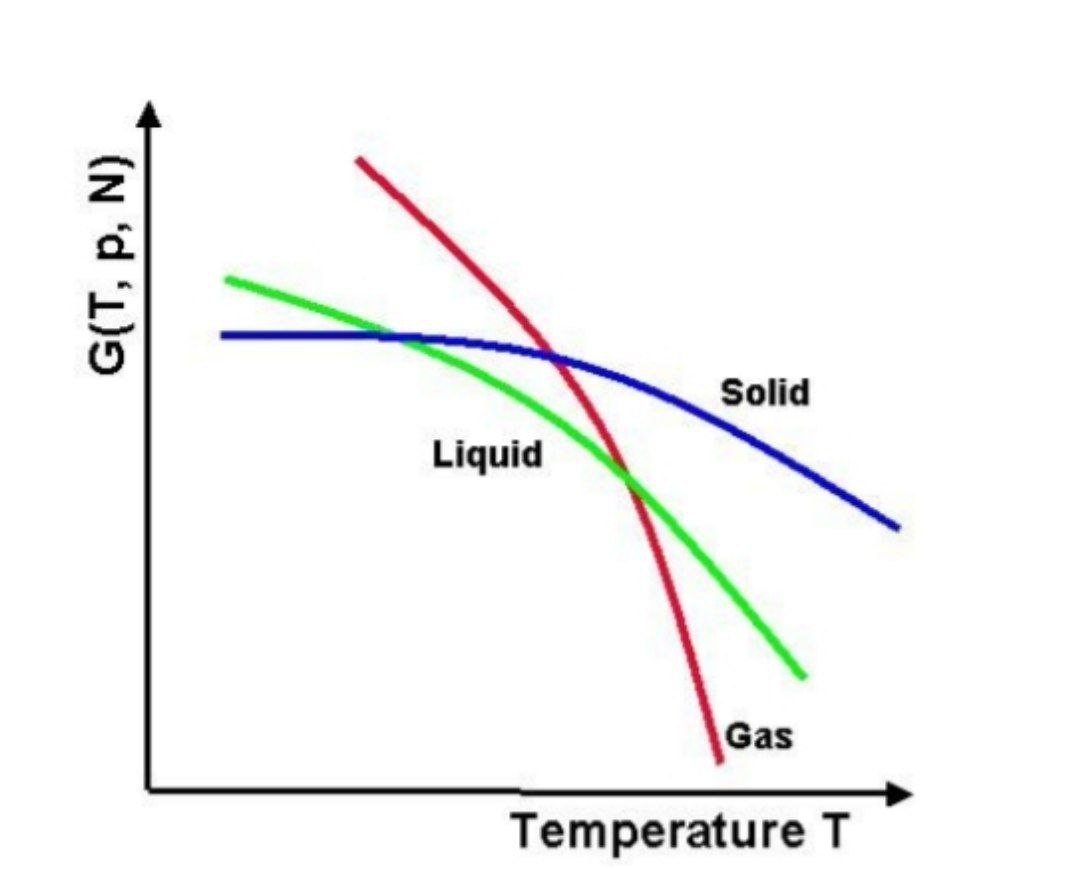
\includegraphics[width = 0.6\textwidth]{img41}
    \caption{Esempio dell'andamento dell'energia libera di Gibbs in funzione della temperatura per fasi solide, liquide e gassose. Fornita da Andrea Fiori.}
    \labfig{img41}
\end{figure}

Un altro esempio è anche la modalità in cui gli elettroni vanno a riempire gli orbitali atomici o la rottura dei domini magnetici, che avviene quando la temperatura supera la temperatura di Curie: in questo caso prevale l’entropia e quindi, un sistema disordinato.

Infine, anche nel caso delle soluzioni solide si risente dell’effetto dell’entropia: considerando ad esempio gli ottoni, cioè soluzione solide di rame e zinco, si può vedere come a basse temperature si formi un ottone del primo tipo, dove lo zinco è solubile al 39\%: si tratta di una lega duttile, malleabile e lavorabile. Se si supera il limite di solubilità, si formano le fasi $\beta$ e $\beta$’. Al 50\% circa di Zn, $\beta$’ è una soluzione solida ordinata, cioè ha un reticolo CCC.\\
Se si superarono la temperatura di 454°C, la soluzione solida diventa disordinata, pur non variando la composizione chimica.

\begin{marginfigure}[-5cm]
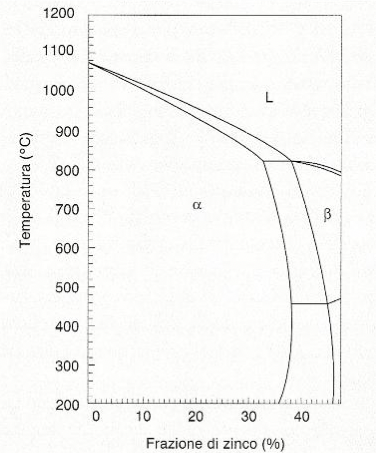
\includegraphics{images/img23.png}
\caption{Porzione del diagramma di fase Cu - Zn a basse percentuali di Zn}
\labfig{img23}
\end{marginfigure}

\subsection{Vacanze}

Le vacanze sono difetti di reticolo puntuali e sono caratterizzate dalla mancanza di un atomo in una posizione reticolare dove, invece, dovrebbe essere presente. Le vacanze sono fondamentali perché facilitano il moto di diffusione (per vacanze) ed inoltre, hanno la proprietà di essere termodinamicamente prevedibili.\\
Le vacanze possono essere create dal passaggio di atomi dall’interno del cristallo verso la superficie. Possono muoversi dentro il cristallo in conseguenza del salto di un atomo da una posizione intorno alla vacanza, entro la vacanza stessa.

Per creare una vacanza serve un certa quantità di energia, necessaria a:
\begin{enumerate}
    \item vincere le forze esercitate dagli atomi sull'atomo che si muove;
    \item compiere il movimento stesso.
\end{enumerate}

Il lavoro, quindi l’energia, è fornito dalle vibrazioni termiche del reticolo cristallino, le quali dipendono dalla temperatura.

L’entropia è una funzione probabilistica ed una misura delle possibili configurazioni ordinate di un sistema, le quali convergono verso il minimo di energia. Le possibilità di evoluzione di un sistema sono, in genere:
\begin{itemize}
    \item miscela, un insieme di atomi con un certo numero di vacanze;
    \item reticolo perfetto con vuoti.
\end{itemize}


La presenza di vacanze incrementa l’entropia della miscela a causa di due contributi: l’entropia intrinseca e l’entropia di miscela, definita come
\begin{equation*}
    \mathrm{S_m=-(n_0-n_v)K\Big[\frac{n_v}{n_0+n_v}\ln{\Big(\frac{n_v}{n_0+n_v}\Big)}+\frac{n_0}{n_0+n_v}\ln{\Big(\frac{n_0}{n_0+n_v}\Big)}}\Big]
\end{equation*}

Dove K è la costante di ltBoltzmann ($\mathrm{K = 1,380649\cdot 10^{-23}JK^{-1}}$), $\mathrm{n_0}$ è il numero di atomi e $\mathrm{n_v}$ quello di vacanze.

Quindi, possiamo modificare l’espressione dell’energia libera di Gibbs per le vacanze:
\begin{equation*}
    \mathrm{\bold{G_m=n_vW_vT\Delta S_m}}
\end{equation*}

con $\mathrm{W_v}$ lavoro necessario per formare una vacanza e $\mathrm{\Delta S_m}$ è l’entropia della miscela che dà un’idea di quale sistema è più probabile che si verifichi.\\
Quindi, il numero delle vacanze cercherà di raggiungere per ogni temperatura un valore corrispondente a un minimo di $\mathrm{G_v}$.\\
La stessa trattazione per le vacanze può anche valere anche per quanto riguarda la quantità di lavoro necessaria per introdurre gli atomi di carbonio nel reticolo del ferro. L'espressione darà la solubilità del carbonio nel ferro, ottenendo cioè un tratto del diagramma di stato Fe-C. Il diagramma Fe-C è la sovrapposizione di quello ferro-cementite e ferro-grafite.\\
Dal punto di vista termodinamico, la presenza di cementite sarà favorita rispetto a quella di grafite, in quanto quest’ultima ha energia di attivazione molto più alta rispetto alla prima.

\section{Metodi di separazione}

In genere i metalli, siccome sono molto reattivi con l'ossigeno (sono cioè facilmente ossidabili, con alcune importanti eccezioni), vengono rinvenuti in natura sotto forma di ossidi all'interno dei minerali. È quindi necessario separare il metallo dall'ossigeno. La difficoltà di questo particolare processo è la causa dell'utilizzo di metalli particolari in epoche storiche differenti: mentre il rame può essere separato dall'ossigeno in fornaci primitive (età del rame) l'alluminio è, in questo senso, una pigna in culo.\sidenote{Il processo era talmente costoso che il servizio buono della reggia di Versailles era in alluminio.}\\
Lo studio dei metodi di separazione consiste nel valutare come varia l’energia dell’ossido al variare della temperatura.

\begin{equation*}
    \mathrm{MeO_{(solido)}\leftrightarrows Me_{(solido)}+O_{(gassoso)}}
\end{equation*}

Aumentando la temperatura, i sistemi disordinati sono più stabili, quindi l’ossido tende a dissociarsi. A basse temperature prevale la presenza dell’ossido, mentre ad alte temperature prevale la reazione di dissociazione.

Dal punto di vista cinetico, ad alte temperature è favorita la reazione di ossidazione del metallo. Dal punto di vista termodinamico, gli ossidi tendono a dissociarci in metallo e ossigeno all’aumentare della temperatura poiché aumenta l’energia libera dell’ossido, in quanto è meno stabile.\\
Diagrammando l’energia libera in funzione della temperatura, si ottengono curve monotone crescenti, che, in scala logaritmica, sono delle rette.

Nel caso dell’energia di formazione di ossidi di rame o alluminio, possiamo avere due casi:
\begin{enumerate}
    \item $\mathrm{3Cu+Al_2O_3\to2Al+3CuO}$
    \item $\mathrm{2Al+3CuO\to3Cu+Al_2O_3}$
\end{enumerate}

La reazione che avviene è la seconda, in quanto l’energia di formazione dell’ossido di alluminio è minore di quella dell’ossido di rame. Non è quindi possibile che il rame riduca l’ossido di alluminio (primo caso).\\
Osservando la figura, notiamo che la curva dell’ossido di alluminio è stabile e sta sempre al di sotto della curva dell’ossido di rame: quindi, è l’alluminio che riduce l’ossido di rame.

Tuttavia, nel ferro, l’ossigeno libero si riassopita con il metallo e si forma nuovamente l’ossido. Per conciliare il diverso comportamento termodinamico e cinetico, bisogna, quindi, introdurre un ulteriore elemento che sia in grado di reagire con l’ossigeno, che nel caso della produzione industriale deve costare poco, essere reperibile e deve avere maggiore affinità con l’ossigeno del ferro stesso.\\
Tale elemento è il \textbf{carbonio}:
\begin{itemize}
    \item $\mathrm{FeO+C\to Fe+CO_{(gassoso)}}$
    \item $\mathrm{2FeO+C\to2Fe+CO_{2(gassoso)}}$
\end{itemize}

Dal punto di vista termodinamico:
\begin{itemize}
    \item  $\mathrm{2CO\to2C+O_2}$
    \item $\mathrm{CO_2\to C+O_2}$
\end{itemize}

Nel caso del monossido di carbonio, cioè nel primo caso, il sistema più disordinato è quello dell’ossido, in quanto abbiamo due molecole di gas prima che la dissociazione avvenga: il sistema indissociato è il più stabile. Di solito, proprio il sistema dissociato è quello a entropia maggiore. Nel diagramma G-T si ha, infatti, una curva decrescente.

Nel caso, invece, dell’anidride carbonica, cioè nel secondo caso, si ottiene una molecole di gas da una molecola di gas. La retta in questo è quasi orizzontale, in quanto la reazione non dipende dalla temperatura.

Si può costruire il \textbf{diagramma di Ellingham-Richardson} (\reffig{img24}): le rette che si ottengono saranno delle spezzate a causa del cambiamento dello stato di aggregazione.
\begin{figure}[!hbt]
    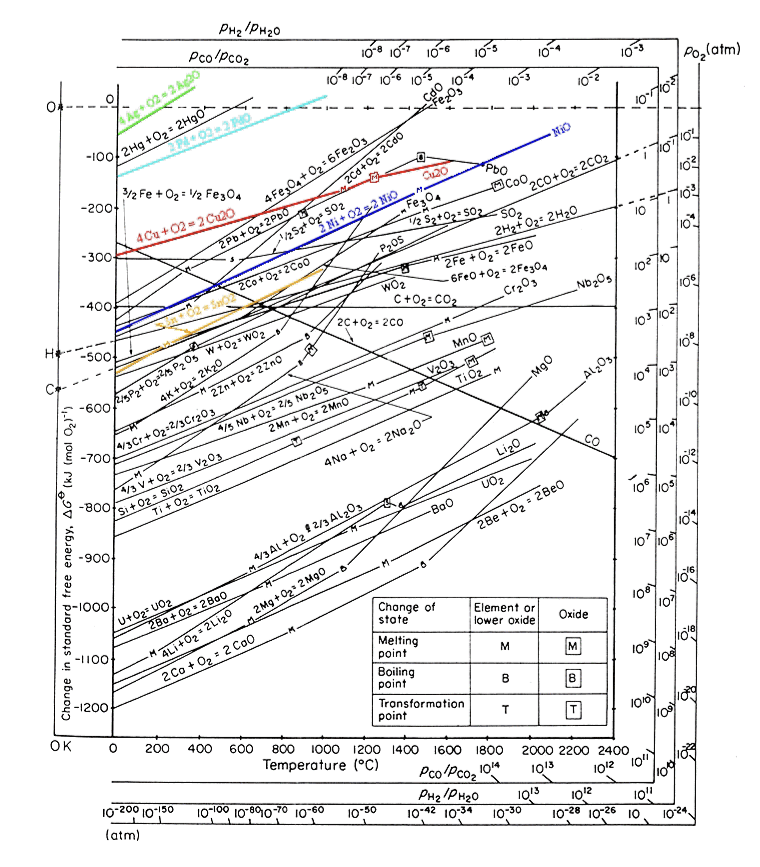
\includegraphics[width=1\textwidth]{images/img24.png}
    \caption{diagramma di Ellingham-Richardson}
    \labfig{img24}
\end{figure}

Si noti che in questo grafico è molto facile ridurre l’ossido di rame: da temperature basse (80°C), il monossido di carbonio è più stabile dell’ossido di rame e quindi, semplicemente scaldando delle cupropiriti (il minerale del rame), si ha la formazione di \textbf{rame metallico}.

La temperatura a cui il ferro si riduce, invece, si aggira attorno sui 1000°C: per raggiungere queste temperature vi è bisogno un camino per il tiraggio e del mantice per rinvigorire le reazioni di combustione. In altre parole, sono necessari i forni soffiati, dove il carbonio (ottenuto in origine tramite carbone prodotto da combustione di legna) riesce così, raggiungendo temperature elevate, a ridurre il ferro. L’acciaio ottenuto artigianalmente si chiama \textit{ferro pudellato}.
\begin{figure}[!hbt]
    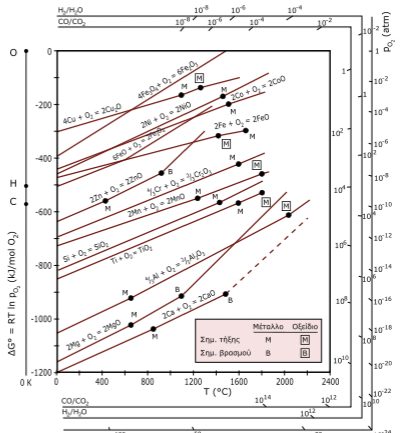
\includegraphics[width=0.8\textwidth]{images/img25.png}
    \caption{}
    \labfig{img25}
\end{figure}

\section{Produzione dell'acciaio}\label{steel_prod}

L’acciaio si può produrre a partire dal minerale (acciaierie a ciclo integrale) o da rottami (acciaierie elettriche).

\index{altoforno}
L’acciaio viene prodotto nell’altoforno: dal basso viene inviata aria, dall’alto invece vengono introdotti il minerale di ferro, il coke e i fondenti.\\
Il minerale deve contenere il 50\% di ferro puro.\\
Il carbone deve essere trasformato in \textbf{coke}, che è carbone quasi puro, molto robusto, in impianti chiamati cokerie. Si dispone il carbone in cataste che vengono bruciate per distillare il carbonio da tutte le impurità. La cokeria è l’impianto veramente inquinante del processo produttivo dell’acciaio.

Il \textbf{fondente}\index{fondente} è principalmente carbonato di calcio (\mathtext{CaCO_3}), che ha principalmente due scopi: il primo è quello di fluidificare la carica, cioè farla scendere con una velocità tale da far avvenire le reazioni, e per eliminare le impurità presenti nel materiale, che poi reagiscono formando le scorie dell’altoforno, chiamate loppe.

Le tre sostanze vengono pre-sinterizzate e omogeneizzate fra loro, per facilitare le reazioni, e poi caricate dall’alto.

\begin{figure}[!hbt]
    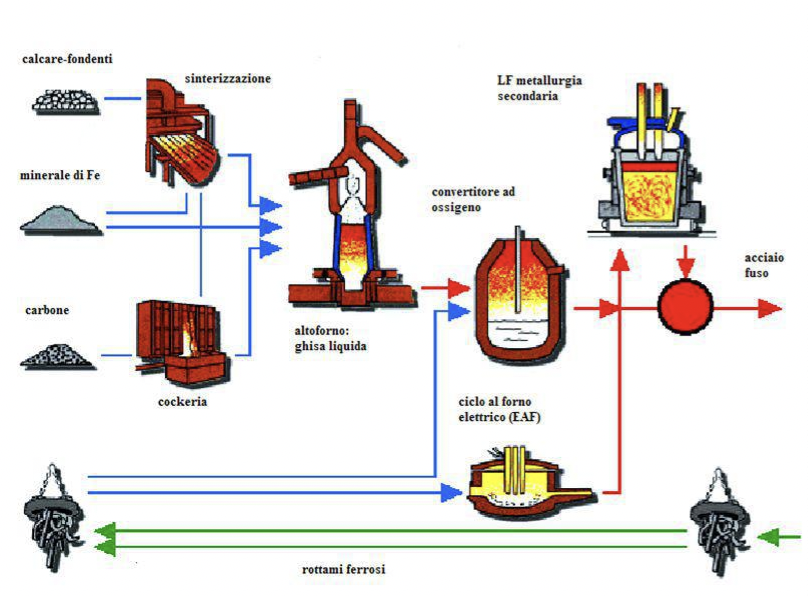
\includegraphics[width=0.8\textwidth]{images/img26.png}
    \caption{Schema della produzione dell'acciaio}
\labfig{img26}
\end{figure}

Nell’\textbf{altoforno} entra dal basso aria calda, riscaldata da quattro serbatoi detti cowpers\index{cowpers}, che sono essenzialmente degli scambiatori di calore.\\
Dato quello che esce dall’altoforno è un insieme di fumi caldi, essi vengono puliti e indirizzati nei cowpers, dove finiscono di bruciare e poi vengono espulsi come gas esausti.\\
La combustione arroventa i cowpers e quindi, viene inviata aria fredda che viene in questo modo pre-riscaldata e poi indirizzata all’altoforno, nella sacca.\\
In particolare, i quattro cowpers funzionano in modo alternato: due si preriscaldando con i gas dell’altoforno, e due invece riscaldano l’aria che deve entrare in altoforno.\\
Ciò che, infine, esce dall'altoforno sono scorie (ossidi di magnesio, di silicio, di zolfo, già presenti nel minerale. Possono essere recuperati per produrre cementi) e metallo di prima fusione, che nel caso specifico è la ghisa con un tenore di carbonio de 4,3\%\sidenote{Ovvero alla concentrazione di carbonio del punto di eutettico}.

Nella sacca arriva l’aria che reagisce con il coke formando monossido di carbonio, che salendo reagisce con il minerale.
In particolare si ha seguente successione di ossidi di ferro: 
\begin{equation*}
    \bold{\mathrm{Fe_2O_3\to Fe_3O_4 \to FeO \to Fe}}
\end{equation*}

Il ferro viene, infine, carburato formando acciaio e il prodotto che esce dall’altoforno è la ghisa.
Per produrre una tonnellata di ghisa, ne occorrono 2 di minerale, 0.9 di coke, 0.4 di fondente e 4 di aria; come prodotti, oltre alla tonnellata di ghisa, ne escono 0.8 di scorie, 5.4 di gas e 0.1 di polvere. Un altoforno può produrre circa 10000 T di ghisa al giorno.\\
Non avendo ferro puro, naturalmente nell’altoforno reagiranno tutti i materiali presenti nel materiale: si aggiungerà del sodio che reagirà con lo zolfo, per eliminare quest’ultimo, poiché non è possibile rimuoverlo all'interno del convertitore.

\begin{figure}[!hbt]
    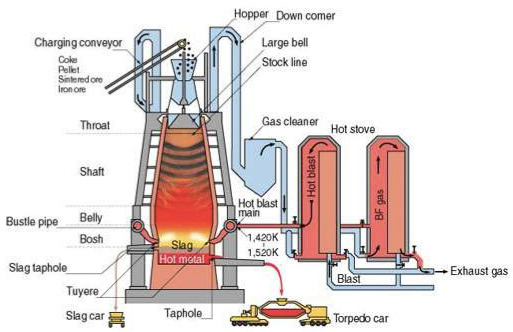
\includegraphics[width=1\textwidth]{images/img27.png}
    \caption{Schema di un altoforno}
    \labfig{img27}
\end{figure}

\index{convertitore}
La ghisa viene trasformata in acciaio tramite un convertitore (che ha una capacità di circa 100 T), dove viene soffiato ossigeno puro e un refrattario basico, per eliminare l’eccesso di silicio e fosforo (che sono acidi). Non può essere usata l’aria perché contiene azoto. Dopodiché il materiale può essere calmato, cioè viene tolto l’ossigeno facendolo reagire con alluminio puro: si ottengono così gli \textbf{acciai calmati}\sidenote{Gli acciai non calmati sono anche detti acciai effervescenti. Sono di scarso interesse industriale perché posseggono caratteristiche meccaniche scarse}.\\
Dopo aver effettuato le opportune aggiunte, l’acciaio viene mandato in colata.\\
Si può avere la \textbf{colata in continuo}: l’acciaio mentre solidifica viene laminato in tubi di rame energicamente raffreddati, ottenendo come prodotto la cosiddetta bramma. Dopodiché si hanno le laminazioni primarie a caldo, \index{decapaggio}il decapaggio\sidenote{Bagni in acido solforico o cloridrico} per eliminare gli ossidi, e infine l’acciaio viene oliato, se è desinato alla vendite diretta, oppure viene laminato a freddo. In quest’ultimo caso, si effettuano successive operazioni di ricottura e di zincatura, per immersione o per elettrodeposizione.\\
La ricottura è necessaria perché il metallo laminato presenta dei gradi di incrudimento eccessivamente elevati. In genere una bramma deve essere tenuta in forno per circa un giorno per poter alleviare questi stress rimanenti. Il processo di ricottura lascia il materiale leggermente corrugato: viene effettuata quindi un'ultima rullatura molto blanda (detta skin milling). È possibile effettuare la ricottura in continuo, "cuocendo" la bramma srotolata in un forno lunghissimo. Questo processo ha il pregio di essere estremamente più veloce rispetto alla ricottura tradizionale, e permette inoltre di effettuare alcuni trattamenti termici già in questa fase.

